\documentclass{standalone}
\usepackage{tikz}
\usetikzlibrary{patterns, positioning}

\begin{document}
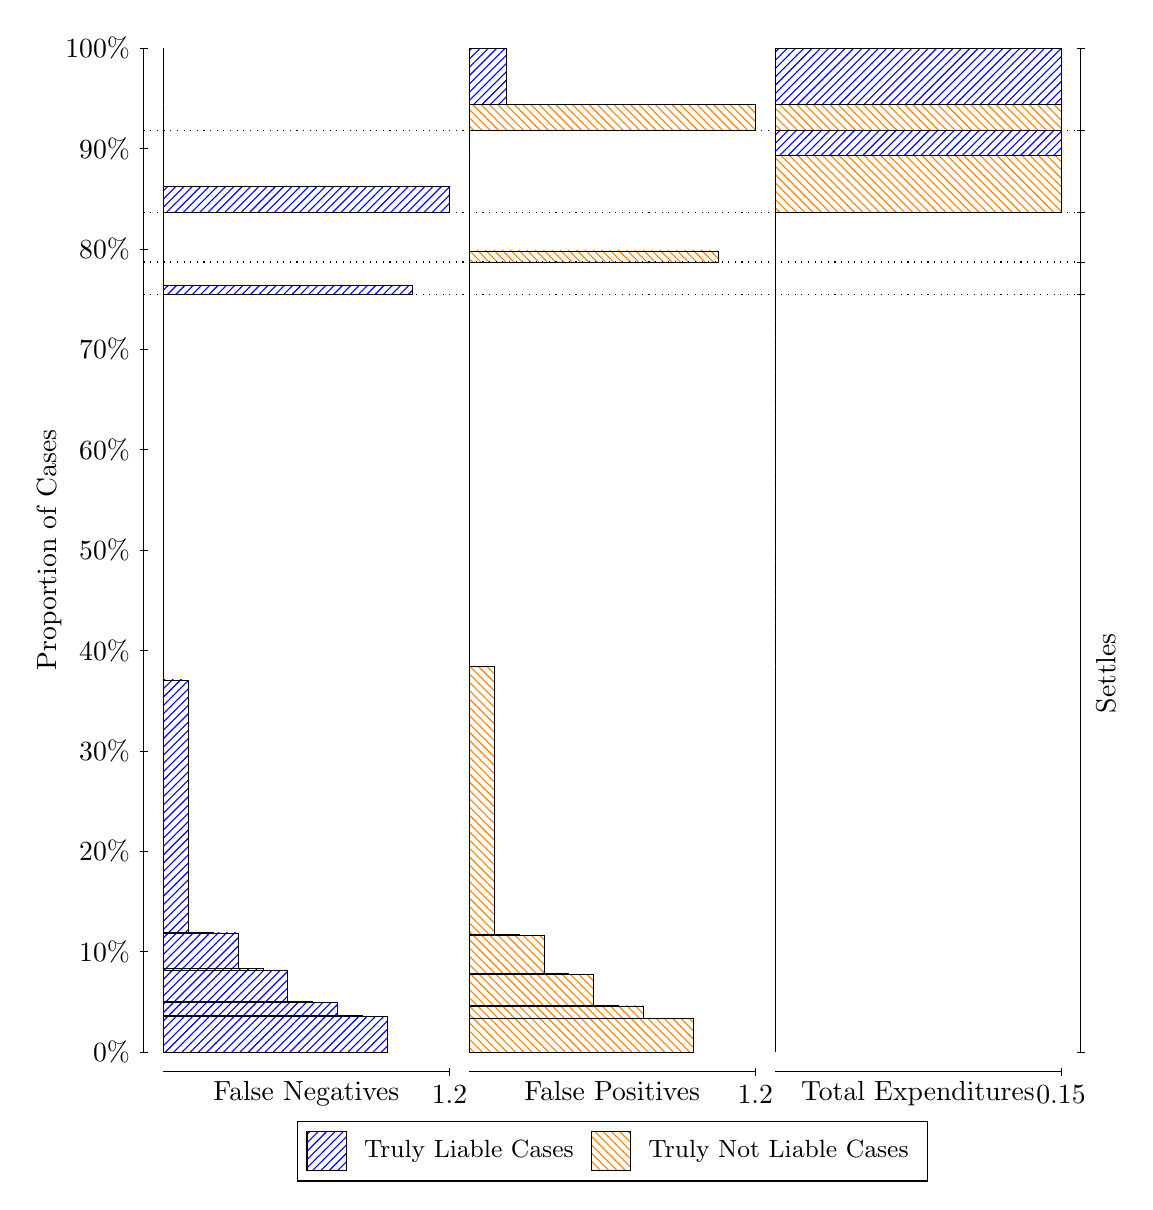
\begin{tikzpicture}
\draw[black, very thin] (1.5,1.75) -- (1.5,14.5);
\node[rotate=90, anchor=center] at (0.3, 8.125) {Proportion of Cases};
\draw[black, very thin] (1.45,1.75) -- (1.55,1.75);
\node[anchor=east] at (1.45, 1.75) {0\%};
\draw[black, very thin] (1.45,3.025) -- (1.55,3.025);
\node[anchor=east] at (1.45, 3.025) {10\%};
\draw[black, very thin] (1.45,4.3) -- (1.55,4.3);
\node[anchor=east] at (1.45, 4.3) {20\%};
\draw[black, very thin] (1.45,5.575) -- (1.55,5.575);
\node[anchor=east] at (1.45, 5.575) {30\%};
\draw[black, very thin] (1.45,6.85) -- (1.55,6.85);
\node[anchor=east] at (1.45, 6.85) {40\%};
\draw[black, very thin] (1.45,8.125) -- (1.55,8.125);
\node[anchor=east] at (1.45, 8.125) {50\%};
\draw[black, very thin] (1.45,9.4) -- (1.55,9.4);
\node[anchor=east] at (1.45, 9.4) {60\%};
\draw[black, very thin] (1.45,10.675) -- (1.55,10.675);
\node[anchor=east] at (1.45, 10.675) {70\%};
\draw[black, very thin] (1.45,11.95) -- (1.55,11.95);
\node[anchor=east] at (1.45, 11.95) {80\%};
\draw[black, very thin] (1.45,13.225) -- (1.55,13.225);
\node[anchor=east] at (1.45, 13.225) {90\%};
\draw[black, very thin] (1.45,14.5) -- (1.55,14.5);
\node[anchor=east] at (1.45, 14.5) {100\%};

\draw[black, very thin] (13.4,1.75) -- (13.4,14.5);
\draw[black, very thin] (13.35,1.75) -- (13.45,1.75);
\node[anchor=west] at (13.35, 1.75) {};
\draw[black, very thin] (13.35,11.371) -- (13.45,11.371);
\node[anchor=west] at (13.35, 11.371) {};
\draw[black, very thin] (13.35,11.782) -- (13.45,11.782);
\node[anchor=west] at (13.35, 11.782) {};
\draw[black, very thin] (13.35,12.416) -- (13.45,12.416);
\node[anchor=west] at (13.35, 12.416) {};
\draw[black, very thin] (13.35,13.458) -- (13.45,13.458);
\node[anchor=west] at (13.35, 13.458) {};
\draw[black, very thin] (13.35,14.5) -- (13.45,14.5);
\node[anchor=west] at (13.35, 14.5) {};

\draw[black, very thin, pattern color=blue, pattern=north east lines] (1.75,1.75) rectangle (4.5935,2.2031);
\draw[black, very thin, pattern color=blue, pattern=north east lines] (1.75,2.2031) rectangle (4.2775,2.21);
\draw[black, very thin, pattern color=blue, pattern=north east lines] (1.75,2.21) rectangle (3.9616,2.3827);
\draw[black, very thin, pattern color=blue, pattern=north east lines] (1.75,2.3827) rectangle (3.6457,2.3896);
\draw[black, very thin, pattern color=blue, pattern=north east lines] (1.75,2.3896) rectangle (3.6457,2.393);
\draw[black, very thin, pattern color=blue, pattern=north east lines] (1.75,2.393) rectangle (3.3297,2.7885);
\draw[black, very thin, pattern color=blue, pattern=north east lines] (1.75,2.7885) rectangle (3.0138,2.8071);
\draw[black, very thin, pattern color=blue, pattern=north east lines] (1.75,2.8071) rectangle (2.6978,3.2622);
\draw[black, very thin, pattern color=blue, pattern=north east lines] (1.75,3.2622) rectangle (2.3819,3.2687);
\draw[black, very thin, pattern color=blue, pattern=north east lines] (1.75,3.2687) rectangle (2.0659,6.4758);
\draw[black, very thin, pattern color=orange, pattern=north west lines] (1.75,6.4758) rectangle (1.75,11.371);
\draw[black, very thin, pattern color=blue, pattern=north east lines] (1.75,11.371) rectangle (4.9094,11.485);
\draw[black, very thin, pattern color=orange, pattern=north west lines] (1.75,11.485) rectangle (1.75,11.782);
\draw[black, very thin, pattern color=orange, pattern=north west lines] (1.75,11.782) rectangle (1.75,11.923);
\draw[black, very thin, pattern color=blue, pattern=north east lines] (1.75,11.923) rectangle (1.75,12.416);
\draw[black, very thin, pattern color=blue, pattern=north east lines] (1.75,12.416) rectangle (5.3833,12.741);
\draw[black, very thin, pattern color=orange, pattern=north west lines] (1.75,12.741) rectangle (1.75,13.458);
\draw[black, very thin, pattern color=orange, pattern=north west lines] (1.75,13.458) rectangle (1.75,13.783);
\draw[black, very thin, pattern color=blue, pattern=north east lines] (1.75,13.783) rectangle (1.75,14.5);
\draw[black, very thin, pattern color=orange, pattern=north west lines] (5.6333,1.75) rectangle (8.4768,2.1725);
\draw[black, very thin, pattern color=orange, pattern=north west lines] (5.6333,2.1725) rectangle (8.1609,2.1758);
\draw[black, very thin, pattern color=orange, pattern=north west lines] (5.6333,2.1758) rectangle (7.8449,2.3357);
\draw[black, very thin, pattern color=orange, pattern=north west lines] (5.6333,2.3357) rectangle (7.529,2.3448);
\draw[black, very thin, pattern color=orange, pattern=north west lines] (5.6333,2.3448) rectangle (7.213,2.7353);
\draw[black, very thin, pattern color=orange, pattern=north west lines] (5.6333,2.7353) rectangle (6.8971,2.7404);
\draw[black, very thin, pattern color=orange, pattern=north west lines] (5.6333,2.7404) rectangle (6.8971,2.7509);
\draw[black, very thin, pattern color=orange, pattern=north west lines] (5.6333,2.7509) rectangle (6.5812,3.2344);
\draw[black, very thin, pattern color=orange, pattern=north west lines] (5.6333,3.2344) rectangle (6.2652,3.245);
\draw[black, very thin, pattern color=orange, pattern=north west lines] (5.6333,3.245) rectangle (5.9493,6.6456);
\draw[black, very thin, pattern color=blue, pattern=north east lines] (5.6333,6.6456) rectangle (5.6333,11.371);
\draw[black, very thin, pattern color=orange, pattern=north west lines] (5.6333,11.371) rectangle (5.6333,11.668);
\draw[black, very thin, pattern color=blue, pattern=north east lines] (5.6333,11.668) rectangle (5.6333,11.782);
\draw[black, very thin, pattern color=orange, pattern=north west lines] (5.6333,11.782) rectangle (8.7928,11.923);
\draw[black, very thin, pattern color=blue, pattern=north east lines] (5.6333,11.923) rectangle (5.6333,12.416);
\draw[black, very thin, pattern color=orange, pattern=north west lines] (5.6333,12.416) rectangle (5.6333,13.133);
\draw[black, very thin, pattern color=blue, pattern=north east lines] (5.6333,13.133) rectangle (5.6333,13.458);
\draw[black, very thin, pattern color=orange, pattern=north west lines] (5.6333,13.458) rectangle (9.2667,13.783);
\draw[black, very thin, pattern color=blue, pattern=north east lines] (5.6333,13.783) rectangle (6.1072,14.5);
\draw[black, very thin, pattern color=orange, pattern=north west lines] (9.5167,1.75) rectangle (9.5167,6.6456);
\draw[black, very thin, pattern color=blue, pattern=north east lines] (9.5167,6.6456) rectangle (9.5167,11.371);
\draw[black, very thin, pattern color=orange, pattern=north west lines] (9.5167,11.371) rectangle (9.5167,11.668);
\draw[black, very thin, pattern color=blue, pattern=north east lines] (9.5167,11.668) rectangle (9.5167,11.782);
\draw[black, very thin, pattern color=orange, pattern=north west lines] (9.5167,11.782) rectangle (9.5167,11.923);
\draw[black, very thin, pattern color=blue, pattern=north east lines] (9.5167,11.923) rectangle (9.5167,12.416);
\draw[black, very thin, pattern color=orange, pattern=north west lines] (9.5167,12.416) rectangle (13.15,13.133);
\draw[black, very thin, pattern color=blue, pattern=north east lines] (9.5167,13.133) rectangle (13.15,13.458);
\draw[black, very thin, pattern color=orange, pattern=north west lines] (9.5167,13.458) rectangle (13.15,13.783);
\draw[black, very thin, pattern color=blue, pattern=north east lines] (9.5167,13.783) rectangle (13.15,14.5);
\draw[black, dotted] (1.5,11.371) -- (13.4,11.371);
\draw[black, dotted] (1.5,11.782) -- (13.4,11.782);
\draw[black, dotted] (1.5,12.416) -- (13.4,12.416);
\draw[black, dotted] (1.5,13.458) -- (13.4,13.458);
\draw[black, very thin] (1.75,1.5) -- (5.3833,1.5);
\node[anchor=north] at (3.5667, 1.5) {False Negatives};
\draw[black, very thin] (5.3833,1.45) -- (5.3833,1.55);
\node[anchor=north] at (5.3833, 1.45) {1.2};

\draw[black, very thin] (5.6333,1.5) -- (9.2667,1.5);
\node[anchor=north] at (7.45, 1.5) {False Positives};
\draw[black, very thin] (9.2667,1.45) -- (9.2667,1.55);
\node[anchor=north] at (9.2667, 1.45) {1.2};

\draw[black, very thin] (9.5167,1.5) -- (13.15,1.5);
\node[anchor=north] at (11.333, 1.5) {Total Expenditures};
\draw[black, very thin] (13.15,1.45) -- (13.15,1.55);
\node[anchor=north] at (13.15, 1.45) {0.15};

\node[black, centered, rotate=90] at (13.72, 6.5607) {Settles};





\draw (7.449999999999999,1.5) node[draw=none] (baseCoordinate) {};
\begin{scope}[align=center]
        \matrix[scale=0.5, draw=black, below=0.5cm of baseCoordinate, nodes={draw}, column sep=0.1cm]{
            \node[rectangle, draw, minimum width=0.5cm, minimum height=0.5cm, pattern=north east lines, pattern color=blue] {}; &
            \node[draw=none, font=\small] (B) {Truly Liable Cases}; &
            \node[rectangle, draw, minimum width=0.5cm, minimum height=0.5cm, pattern=north west lines, pattern color=orange] {}; &
            \node[draw=none, font=\small] (B) {Truly Not Liable Cases}; \\
            };
\end{scope}

\end{tikzpicture}
\end{document}